\documentclass[..thesis.tex]{subfiles}

\begin{document}
\subsection{Overview}


To explain the role of device drivers, lets introduce two common devices that are usable on computers running a Linux operating system.

First of them is \textit{/dev/tty}, a device that represents the terminal controlling the current process \cite{torvalds_linux}. Opening a terminal in Linux and writing to the device results in the text being displayed in the terminal. One can try this with the following command: 

\textit{echo "Hello" > /dev/tty}.\toask{ Too detailed example? Can skip commands if they do not add value.}
 
Second device we will introduce is \textit{/dev/null}, a device that discards any data sent to it. So, redirecting text to this device has no effect.
One can send text to the device as follows:

\textit{echo "Hello" > /dev/null}.

Although the two devices act differently, they both can be used the same way -- we can redirect text to them (and redirect text from them). This allows us to group the two devices together when reasoning about how to use them. The benefits of this are far greater when the number of devices that can be grouped together grows.

The role of Linux device drivers is to enable such groupings that can contain arbitrary amount of devices.

This is done by enabling access to the devices via a small set of well-defined interfaces that other parts of Linux kernel can make use of. 

In this paper we will focus on a subset of device drivers called \textit{character (char) device drivers}. Character device drivers allow unbuffered access to the underlying ``hardware''. Both of the drivers for the example devices are char drivers.

\subsection{Interface of a character device driver}

Devices are exposed to end user as entries in the file system and so it is natural to use the same terminology for talking about device drivers operations as about normal file operations. So device drivers expose end points for \textit{reading}, \textit{writing to}, \textit{opening} and \textit{releasing} the device. This list is not exhaustive\cite[include/linux/fs.h]{torvalds_linux}, but it is not necessary for a driver to expose them all.

As a running example we will introduce the driver \textit{Counter}. \textit{Counter} keeps track of the difference between how many times kernel has read from it and how many times kernel has written to it \footnote{The full source code is avalible in Appendix \ref{A:example-driver}}.

In the following code snippet, the parameters of the functions are omitted as they are not relevant for this example.



\begin{lstlisting}[language=C,style=def]
static ssize_t file_read(...){
    ++i;
    printk("++i, new value:: %d \n",i);
    ...
}

static ssize_t file_write(...){
    --i;
    printk("--i, new value: %d \n",i);
    ...
}

static int file_open(...)
{
    printk( "Opening device \n");
    return 0;
}

static int file_release(...){
    printk( "Closing device \n");
    return 0;
}


\end{lstlisting}
\tosup{\sout{Meaning of the return types: what is this ``s''?}}
\todisc{ ``s'' was left over from copy-pasteing from the working driver, does not make sense here after simplification. The total amount of bytes either read or written. As I have left out the buffer argument where one actually would write to, I have removed it from here. Can add the code for the driver into the appendix?}

\toadd{\sout{Add code of the driver to appendix}}

The \textit{read} function increases the global counter by one, while \textit{write} function of decreases it by one. Both the \textit{open} and \textit{release} functions only output info to kernel log.

When a user reads from a file that exposes the driver, one can see that the file was opened, read and then closed. For a concrete example,
\textit{head -c 1 < counter} produces the following entries in the kernel log:

\begin{lstlisting}[language=sh,style=def]
vootele kernel: Opening file 
vootele kernel: Increasing i, new value: 1 
vootele kernel: Closing file 
\end{lstlisting}

And similarly, when writing to the file, for example with \textit{echo hi > my-driver} then the file is opened, written into and then closed.


Drivers expose the device to the kernel via \textit{file operations} structure. When registering a driver to the kernel, the \textit{file operations} structure is registered with kernel and kernel can invoke any of the methods specified in the structure.

The \textit{file operations} structure of \textit{Counter} is 

\begin{lstlisting}[language=c,style=def]
static struct file_operations f_ops = {
  .write   = file_write,
  .read    = file_read,
  .open    = file_open,
  .release = file_close,
};
\end{lstlisting}

Device drivers also expose \textit{init} and \textit{exit}, which kernel can use to register and de-register the device driver. In case of \textit{Counter}, registering the device initializes the counter $i$ to zero and then registers the \textit{file operations}. 

\tocomment{ Do not want to inline these two, the exit has no value (only memory released), init has calls to library functions that do not make sense  on the quick glance.}



\toadd{\sout{What are they, interface they expose}, \sout{life-cycle}} \tocomment{ taken to concurrency section}
\toask{ Something missing? Also, I have inlined a lot of code here. I think it does serve its purpose -- makes the paper less dense . Also, I use this as a running example, so I will be referring back to it. Linux commands could be cut, for me they bridged the cap between the devices and my experience as Linux user, but they will not do that for someone who has very little experience with Linux (?). Ideas welcome.  }
\tosup{\sout{I don't like the interleaving of single sentence text with the code. I would put all the device code in a single listing, or at least group open/close and read/write. More importantly, very short commands that are embedded in the text should be inlined. This head c 1 < counter with text continuing on the next line is not very nice.}}
\todisc{Agreed, the listing look mediocre as well, will see if I can get them to look better. The file operations are in the one listing now and the commands are inlined.}

\tocomment{inlined with interface description}

\toadd{ \sout{ Concrete example, what it does, exposed interface, snippets of interesting parts of code. Best case, something that contains actual concurrency issue (or something that gets flagged as one).  Hopefully a running example that can be turned back to}} 
\tocomment{Running with my own example, does not do much, but easy enough to show code inline and that has obvious concurrency issues.The fonts are also inconsistent with the previous section.}

\subsection{Data-races in device drivers}

\toadd{\sout{lifecycle}}

When registering our driver, we exposed multiple endpoints to the kernel. From that moment onwards, kernel can invoke any of the registered methods, at any time, until the driver is de-registered. 

\toguide{ Why are data-races relevant for Linux device drivers?}

The multitude of entry points to the programs and lack of control over when they are entered makes avoiding data races a challenge when writing Linux device drivers. 

For an example of a data-race in device drivers, it is quite obvious that when one writes to a ``device'' exposed by the example driver concurrently, then the value of counter after all the write operations is not determined -- it is easily possible that between the read and write operations of the counter, its value gets updated.

To be more concrete, on Figure \ref{fig:driver-race} is a snippet of kernel log after running a script \footnote{Available in Appendix \ref{A:test-script}} that reads and writes to the example driver in a loop that
runs 10 000 times in 3 proccesses at the same time. As the read operation increases $i$ and write operation decreases it, the expected value without data-races would have been $0$.


\tocomment{ In presentation, I can easily start a script and show that this is the case. I do not that this translates to writing very well, I could Monte Carlo it and and the distribution table of the final value of the counter, but I think it would be too much noise? Feedback appreciated on this one.}

\tosup{\sout{It would be helpful to discuss one concrete case where the race happens.  Maybe a screenshot of the unexpected output?} }
\todisc{Added.}

\begin{figure}[H]
\centering
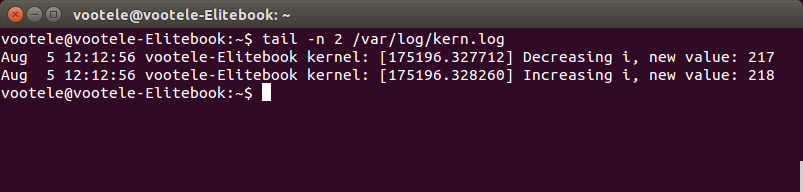
\includegraphics[width=0.9\textwidth]{driver-race}
\caption{Snippet from kernel log after data-race in an example device driver}
\label{fig:driver-race}
\end{figure}


\toguide{ There are ways around them, right?}

To avoid data-races, Linux kernel offers multiple locking primitives. 

A popular locking primitive is the \textit{spinlock}, which runs a tight loop, inside what it tries to acquire the lock, until it succeeds. This tight loop gives the lock its name. Using spinlocks avoids explicitly putting the thread to sleep when acquiring a lock fails. If it is known that lock is held only for a very short time then the computational cost of putting a thread to sleep and then later awakening it out-weights the extra CPU cycles used by the tight loop of a spinlock.

Spinlocks also offer a lock that differentiates between reads and writes, allowing multiple concurrent reads.

One of the most commonly used locking primitives is the \textit{mutually exclusive lock} (mutex). It also the one that one should use, if possible \cite[Documentation/locking/mutex-design.txt]{torvalds_linux}. The older implementations of mutex put the thread to sleep if acquiring the lock failed whereas the current implementation is also capable of spinning for a limited time before resorting to explicitly putting the thread to sleep.

\tosup{\sout{Wait, spinlock blocks until the lock has been acquired. What do you mean by blocking? This typically refers to giving up the CPU. Spinlocks do not block, they spin!}}
\todisc{Think I meant ``block'' as ``blocking IO'', but that would be kinda pointless as well. Rewritten.}

To eliminate a possible data race from our example driver, we could add a lock to the driver and acquire it on every read and write operation. With the added lock, the read operation would look as follows:

\begin{lstlisting}[language=C,style=def]
static ssize_t file_read(...){
    mutex_lock(&my_mutex);
    ++i;
    printk("++i, new value: %d \n",i);
    mutex_unlock(&my_mutex);
    ...
}
\end{lstlisting}

where \textit{my\_mutex} is a static mutex.

After adding the same locking pattern to write operations, data-races will no longer plague the example driver.

\tocomment{ I like examples, but I think going over write AND read would be overkill. Some doubts on whether this example is helpful, comments welcome.}


\toguide{Are there any other ways?}

There are also alternatives to straightforward locking that one can use when writing Linux device drivers to eliminate data races, such as \textit{seqlocks} and \textit{read-copy-update}. These fall outside the scope of this paper, as they are rarely used compared to traditional locking and as of now, static analysis tools do not offer much support for them. 


\subsection{Impact of data races in device drivers}

We have seen that data races are a real possibility in device drivers and also that there are ways to protect oneself against them. 

\toguide{ Why are the data-races prevalent?}

As previously discussed, Linux device drivers usually have multiple entry points and no control over when they are entered. Also, the device drivers are written in C, a low level language, that makes reasoning about them quite challenging. Furthermore, quite often the person writing a driver is an expert on the device that the driver is for, and not so much an expert on Linux device drivers themselves. This makes correct usage of constructs that help to avoid data races difficult and error-prone.

\toguide{ How common are the data races?}

\toadd{ \sout{Studies showing that this is indeed an issue -- drivers are buggy and have concurrency bugs. Hard to discover, get shipped quite often.}}


Empirical studies validate this assertion. In a study done by Chou \textit{et al}. \cite{chou_empirical_2001} it was found that error rates in device drivers are three to seven times higher than in rest of the kernel. 

The situation seems to have become better over time. In the follow-up study conducted by Palix \textit{et al.} \cite{palix_faults_2011}, the error rate in device drivers improved, but drivers still contain the highest number of errors.

In a study done by Ryzhyk and others \cite{ryzhyk_dingo_2009}, out of the 498 bugs found between 2002 and 2008 in 13 selected drivers from Linux device drivers, 93 were concurrency related -- mainly data races or deadlocks. 

Mutilin \textit{et al.} \cite{mutilin_analysis_2012} found that data races are the most common single type of bug, remarkable 5 times more common than deadlocks in Linux device drivers.

It is worth noting that based on \cite{chou_empirical_2001,palix_faults_2011}, the average lifetime of a bug is 18 months, making it quite likely that the bug makes it way to a stable version. 

\toguide{ How bad are they?}

In addition to being common, the bugs in device drivers can cause crashes fatal to the whole system. In Windows XP, 85\% of the reported failures were caused by issues with device drivers \cite{swift_improving_2003}.

The data races are extremely unpleasant in safety critical applications, where their presence could endanger lives. For that reason, the verification requirements of device drivers in safety critical domains (for example aviation or automobile industry) are very rigorous, making the testing process very costly and time-consuming.


\toadd{ Significant part of time it takes to get hardware out, validation and so on. Not sure if I can find anything on this, would need sources } 

\toask{ Tried, without much success, to find case studies where drivers were to root cause. However, I am not sure if this is required, hopefully I have managed to convince reader by now that data races in drivers is a real problem worth tackling?
In any case, I will most likely look for a citation for this in my master thesis, but as of now, I will not spend more time on it.}



\toask{ \sout{ Extra section overkill? Combine with Motivation?} Think it is needed, I am atleast convinced that it is a real problem worth tackling}
\toans{\sout{This is all relevant, but rename section to ``Device Drivers''?}}
\todisc{ Agreed, although I would go without the up-style in section/subsection names if acceptable.}


\end{document}
